%%%%%%%%%%%%%%%%%%%%%%%%%%%%%%%%%%%%%%%%%%%%%%%%%%%%%%%%%%%%%%%%%%%%%%%%
%                                                                      %
%     File: Thesis_Data_Collection.tex                                 %
%     Tex Master: Thesis.tex                                           %
%                                                                      %
%     Author: João C. Godinho                                          %
%     Last modified :  Apr 2018                                        %
%                                                                      %
%%%%%%%%%%%%%%%%%%%%%%%%%%%%%%%%%%%%%%%%%%%%%%%%%%%%%%%%%%%%%%%%%%%%%%%%

\chapter{Data Collection}
\label{chapter:data_collection}

In the current chapter we detail our initial approach to construct a machine learning model that detects malware based on static and dynamic features.
This first approach was to create a dataset of malware and goodware to feed into a ML model.
We start by describing how the training data was collected, followed by how it was analyzed.
We then proceed to label the samples with help of the aforementioned analysis.

%%%%%%%%%%%%%%%%%%%%%%%%%%%%%%%%%%%%%%%%%%%%%%%%%%%%%%%%%%%%%%%%%%%%%%%%
\section{Data Sources}
\label{section:data_sources}

The purpose of this step is to obtain a corpus from which information
about malware and goodware can be extracted.
To minimize any possible bias towards data collection, and to save the overhead time of collecting and analyzing samples, we chose to take advantage of the publicly available reports from Malwr \cite{tool:malwr} service.
As previously mentioned in Section \ref{section:cuckoo}, Malwr is a free online service that does static and dynamic analysis on submitted files using Cuckoo \cite{tool:cuckoo}, which are then accessible in an HTML report.

To enrich our knowledge about samples' \textit{ground truth} we resorted to two other online repositories: \gls{nsrl} \cite{tool:nsrl} and VirusShare.com \cite{tool:virusshare}, these provide metadata (\eg\ MD5 hash) regarding known goodware and malware samples, respectively.
As \gls{nsrl} contains a collection of digital signatures of known, traceable software applications, if a sample is present in this collection, we are more confident it is indeed goodware.
On the other hand, VirusShare.com is a repository of malware samples, hence a sample present in this repository gives us a higher confidence it is indeed malware.

Our data extraction methodology for Malwr and VirusShare.com was based on applying a common data extraction technique, where online data is saved locally or in a central database for further analysis. This technique, called \textit{scraping}, was done using Scrapy \cite{tool:scrapy}, a Python scraping library.

As for the \gls{nsrl} repository, information was provided in textual format, which led us to use Pandas \cite{tool:pandas}, a Python data analysis library, to extract and analyze the data.


%%%%%%%%%%%%%%%%%%%%%%%%%%%%%%%%%%%%%%%%%%%%%%%%%%%%%%%%%%%%%%%%%%%%%%%%
\section{Data Analysis}
\label{section:data_analysis}

The following provide a detailed analysis of the available data sources, done by using Pandas~\cite{tool:pandas}, a Python Data Analysis Library.

%%%%%%%%%%%%%%%%%%%%%%%%%%%%%%%%%%%%%%%%%%%%%%%%%%%%%%%%%%%%%%%%%%%%%%%%
\subsection{High Level Analysis}
\label{subsection:high_level_analysis}

Our first approach was to scrape the list of analysis in Malwr\footnote{Malwr Analysis list [https://malwr.com/analysis/]}.
It is worth noting this scraping did not provide us the full analysis report, only information regarding the type of submission (\eg\ binary, text, archive), its submission date and the sample MD5 hash.

After our initial scraping to obtain a high level view of the available reports, we observed that Malwr had a total of 642,698 submissions, dated between April 16th, 2013 and October 10th, 2016. As can be seen in Figure \ref{fig:samples_count}, there was an increase in sample submission from 2013 up to all time highs in May, June and July of 2014, followed by possibly a downtime period in August 2014.
The service went back up in September 2014, after which it stabilized around 20,000 submissions per month.

\begin{figure}[!htb]
	\centering
	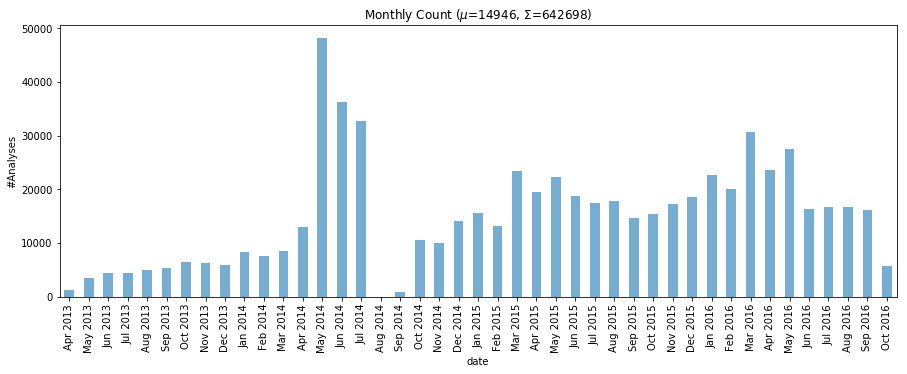
\includegraphics[width=0.95\textwidth]{Figures/samples_count.png}
	\caption[Number of monthly submissions.]{Number of monthly submissions.}
	\label{fig:samples_count}
\end{figure}

Following this initial observation, we measured the percentage of duplicated submissions per month, which vary between 10\% and 20\%, and the percentage of different file types, as shown in Figure \ref{fig:monthly_distributions}.
The file types distribution is interesting, as it shows that executables (\ie\ compiled binary files) took the great majority of submissions up to the end of 2014, after which documents (\eg\ Word, Excel) and text files (\eg\ HTML, JavaScript) started to increase.
As a side observation, this increase might indicate how users are more suspicious of these type of files, given that it is not uncommon to see malware being distributed in documents (under email attachments) and in websites (as JavaScript scripts) in more recent years.

\begin{figure}[!htb]
	\centering
	\begin{subfigmatrix}{2}
		\subfigure[Percentage of duplicated submissions per month (based on MD5).]{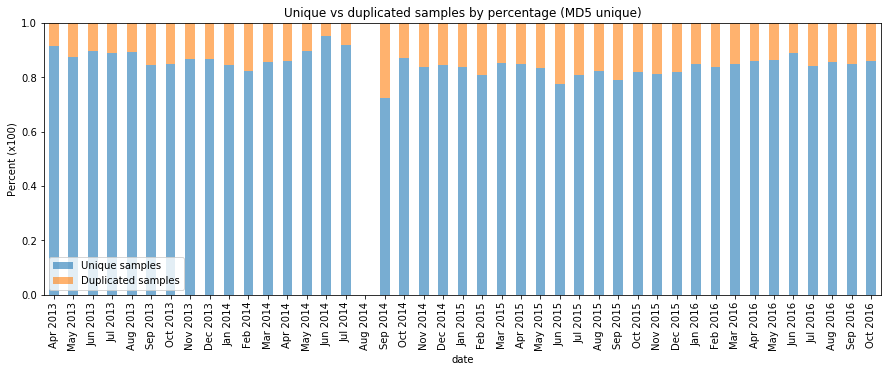
\includegraphics[width=0.95\linewidth]{Figures/samples_dups.png}}
		\subfigure[Distribution of file types per month.]{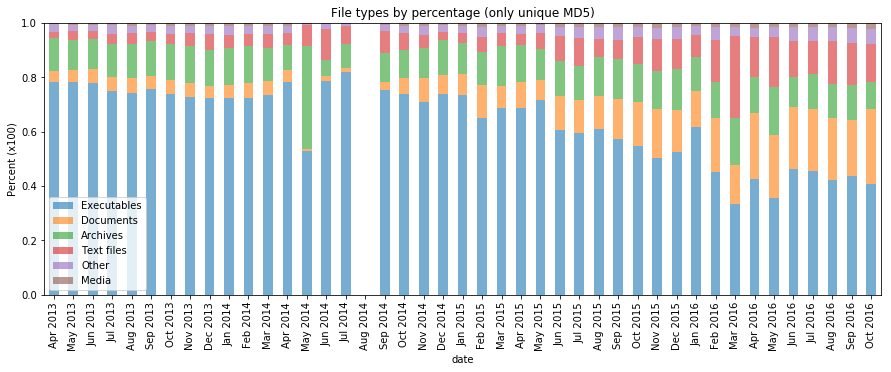
\includegraphics[width=0.95\linewidth]{Figures/samples_types.png}}
	\end{subfigmatrix}
	\caption[Monthly distributions of submissions.]{Monthly distributions of submissions.}
	\label{fig:monthly_distributions}
\end{figure}

Having a better overall understanding on the available reports, and taking into account the limitations of static analysis in \textcolor{red}{Cuckoo} as mentioned in Section \ref{section:cuckoo}, led us to our first data selection criteria: collect reports from \gls{pe} (\eg\ 32bit executables, DLL's) submissions only.
This selection reduces the number of available reports to 388,702 (60.48\% of the total) but enables us to work with more static information.

We went on to extract these reports, again using Scrapy, as HTML files and kept them in a gzip compressed format to save disk space.
A set $\mathcal{R}$ of raw reports, totaling 388,507 submissions was obtained, (different from the
previous amount as some errors could have occurred during scraping) occupying a total of 26GB.

%%%%%%%%%%%%%%%%%%%%%%%%%%%%%%%%%%%%%%%%%%%%%%%%%%%%%%%%%%%%%%%%%%%%%%%%
\subsection{VirusTotal Classifications}
\label{subsection:virustotal_classifications}

As previously mentioned in Section \ref{section:cuckoo}, Malwr aggregates the scan report as provided by VirusTotal (if the sample is already known by VirusTotal), which entails multiple antivirus classifications.
Our next analysis takes advantage of this information to better understand how the samples are labeled and how reliable using the VirusTotal report can be to label our dataset.

After counting the number of different antivirus vendors present in at least one submission, we decided to narrow down to the amount of unique vendors by requiring their presence in at least 95\% of the classified reports.
Doing so guarantees that vendors did not show occasionally and have a strong presence in all classified samples.

By applying this criteria, we narrowed from 97 unique vendors to a smaller set $\VV$ of 38.
This led us to a smaller set $\mathcal{C}\subseteq\mathcal{R}$ of classified reports, which totaled 284,880 submissions. With this new set $\mathcal{C}$ we went on to analyze how reliable the vendors classification is.

Reiterating what was already said, defining and classifying malware is not a trivial task.
The \textit{ground truth} of a sample is hard to obtain, as both antivirus vendors and users disagree on what is malware.
To come to terms with this obstacle, we make use of the classifications given by our set of vendors $\mathcal{V}$ to define a simple malware/goodware criteria: what is the minimum/maximum threshold of positive malware classifications as to label a sample as malware/goodware.

Although this criteria bases itself on a vote policy, adding robustness to the criteria, it also inherits some of the vendors problems: false positives and false negatives. With this in mind, we now aim to understand vendors' accuracy and how they change their classifications.

To study how the classifications vary, we took advantage of the duplicated classified submissions in $\mathcal{C}$. There are 27,798 samples submitted more than once to Malwr, for a total of of 74,916
duplicated submissions $\mathcal{C}_{dups}$ averaging 2.7 submissions per
duplicate.

We now show how we studied the differences between the number of positive classifications on the first and last submission, inspired by Miller's et al. \cite{miller:rev_int} work.

For each duplicated sample in $\mathcal{C}_{dups}$ we counted the number
of positive classifications on the first and last submissions, $\mathcal{P}_f$ and $\mathcal{P}_l$ respectively.
If $\mathcal{P}_f > \mathcal{P}_l$ then we are looking
at a possible false positive (FP), as the number of vendors
classifying the sample as malware decreased.
Conversely, if
$\mathcal{P}_l > \mathcal{P}_f$ we are looking at a potential false negative (FN).
For the case $\mathcal{P}_f = \mathcal{P}_l$ we conclude that vendors are confident regarding their classification for the sample. It is worth noting that there may be cases where $\mathcal{P}_f = \mathcal{P}_l$, but with different vendors (i.e. an equal number of vendors simply switch classification), but given we are looking for a criteria based on a minimum threshold, these cases are not relevant for our analysis.

Figure \ref{fig:dups_frequency} shows the frequency of $\mathcal{P}_l-\mathcal{P}_f$ for each duplicated
sample.
We first note that 44.32\% of duplicated samples change in classification, among which 38.72\% increase its classification (green bars), whereas only 5.61\% decrease (red bars).
There is a clear discrepancy between positive and negative changes, suggesting that vendors favor false negatives (\ie\ increase in positive classifications) over false positives (\ie\ decrease in positive classifications), as also noted by Miller et al. \cite{miller:rev_int}.

\begin{figure}[!htb]
	\centering
	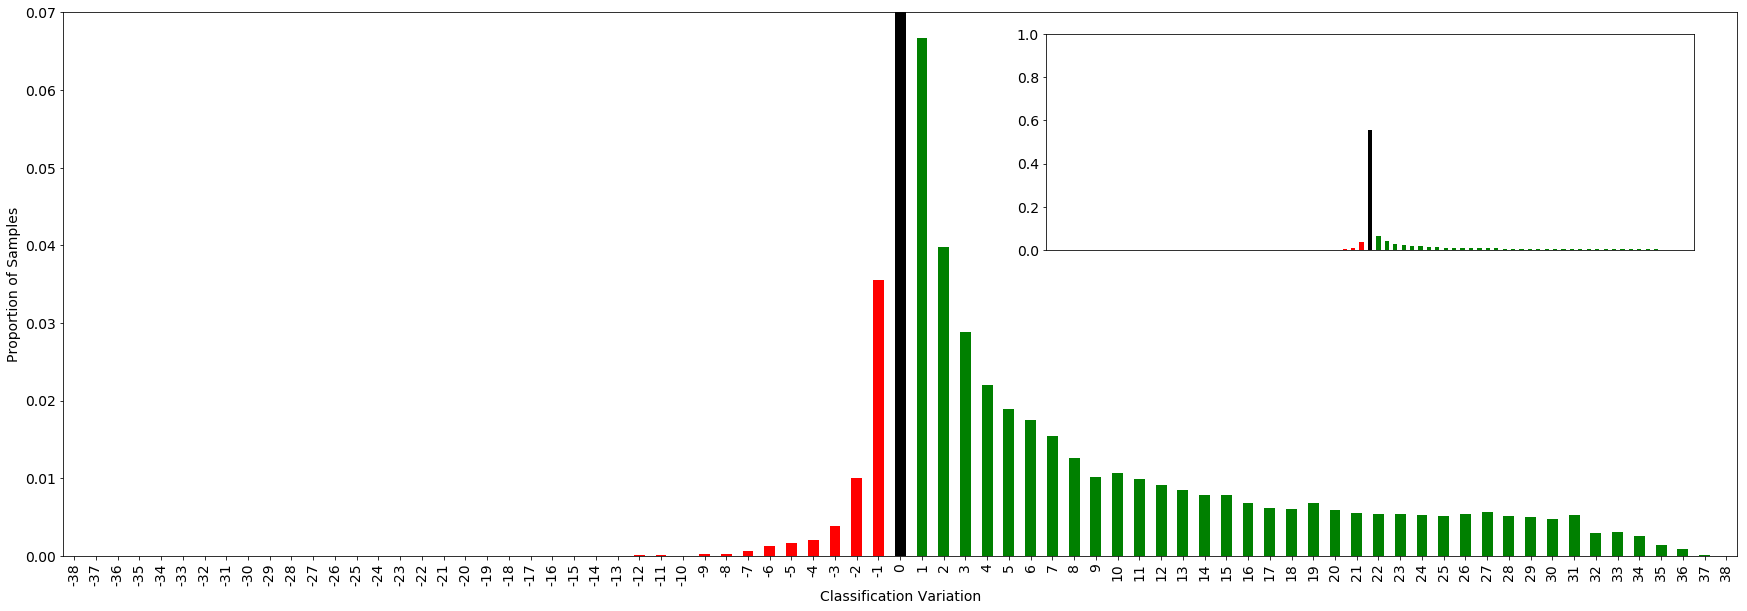
\includegraphics[width=0.95\textwidth]{Figures/dups_frequency.png}
	\caption[Distribution of duplicated samples.]{Distribution of duplicated samples in terms of the changes in the number of
positive classifications between last and first submissions, $\mathcal{P}_l-\mathcal{P}_f$.}
	\label{fig:dups_frequency}
\end{figure}

Another interesting analysis on our samples is understanding the vendors \emph{\gls{dr}} (or True Positive Rate), and \emph{\gls{fpr}}.
Although these formulas are trivially defined respectively as
\begin{eqnarray}
\dr&=&\frac\tp{\#malware}=\frac\tp{\tp+\fn} \\ 
\fpr&=&\frac\fp{\#goodware}=\frac\fp{\tn+\fp}
\end{eqnarray}
we lack ground truth for what is $\#malware$ and $\#goodware$.
To solve this, we must use the available information and propose relative metrics to determine what is positive ($\#malware$) and negative ($\#goodware$).

Our first metric falls back on duplicated submissions again, to define an accuracy metric, $\Madups$. As we have previously shown, 44.32\% of duplicated samples change in classification, which can be translated into vendors acknowledging their own errors.

With that in mind, for each vendor $v\in\VV$, we define a duplicated sample for $v$ (according to $\Madups$) as:
\begin{itemize}
	\item $\tp_v$, \emph{true positive for $v$}, if $v$ classified it positively in both the first and last submissions;
	\item $\tn_v$, \emph{true negative for $v$}, if $v$ classified it negatively in both the first and last submissions;
	\item $\fp_v$, \emph{false positive for $v$}, if $v$ classified it positively in the first submission and negatively in the last submission;
	\item $\fn_v$, \emph{false negative for $v$}, if $v$ classified it negatively in the first submission and positively in the last submission.
\end{itemize}

Figure~\ref{fig:dr_fpr_own} plots each vendors' $\dr_v$ vs.\ $\fpr_v$, under the previously defined metric $\Madups$.
Our first observation is that vendors do acknowledge their own classification errors, as we see a varying $\dr_v$ from 56.82\% to 85.29\%, with a $\fpr_v$ rate ranging from 0.03\% to 6.91\%.
If this was not the case (i.e. vendors would not change their classifications), one would have that $\Pl-\Pf = 0$ for every duplicate and consequently $\dr_v = 1$ and $\fpr_v = 0$, which in turn would mean that all clean samples remain clean, hence $\fn_v=0$, and all malicious samples remain malicious, hence $\fp=0$.
As previously noted, it is apparent that vendors favor \fn\ over \fp,\ as the range for $\fpr_v$ (6.88\%) is much smaller than for $\dr_v$ (28.47\%).

\begin{figure}[!htb]
	\centering
	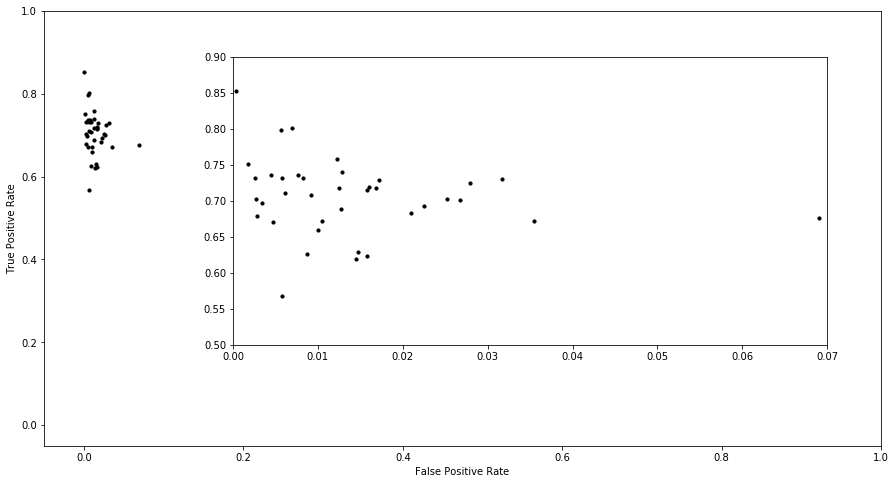
\includegraphics[width=0.95\textwidth]{Figures/dr_fpr_own.png}
	\caption{$\tpr_v$ vs. $\fpr_v$ according to $\Madups$.}
	\label{fig:dr_fpr_own}
\end{figure}

The previous analysis gave us a better understanding on vendors accuracy, but is highly dependent on vendors acknowledging their own errors.
To overcome this dependency, we take a second approach regarding vendors' accuracy, which takes into account our observations from Figure \ref{fig:dups_frequency} and our dataset $\CC$ (instead of $\mathcal{C}_{dups}$), to define another metric $\Mac$.

This new metric $\Mac$ implements a simple minimum/maximum threshold of positive classifications to label a sample as malware/goodware.
Intuitively a sample is classified as goodware according to this metric (\ie\  negative), if every vendor $v\in\mathcal{V}$ classifies it as clean.
To understand if our intuition is sound, we plot Figure~\ref{fig:distribution_clean}, a subset of Figure~\ref{fig:dups_frequency}, showing the frequency $\Pl-\Pf$ for samples that were classified as clean in their first submission (\ie\ samples with $\Pf=0$).
These account for 4,902 samples, 3,741 (76.32\%) of which do not increase in classification.

To arrive at a positive (\ie\ malware) sample definition, we relate Figure \ref{fig:distribution_clean} with Figure \ref{fig:dups_frequency}.
Specifically we want to find a minimum threshold of positive classifications to define a sample as malware.
We chose five as the threshold, observing that percentage of samples that decrease in 5 or more positive classifications is 0.46\%, meaning it is an upper bound for samples that decrease from 5 or more to zero classifications.

\begin{figure}[!htb]
	\centering
	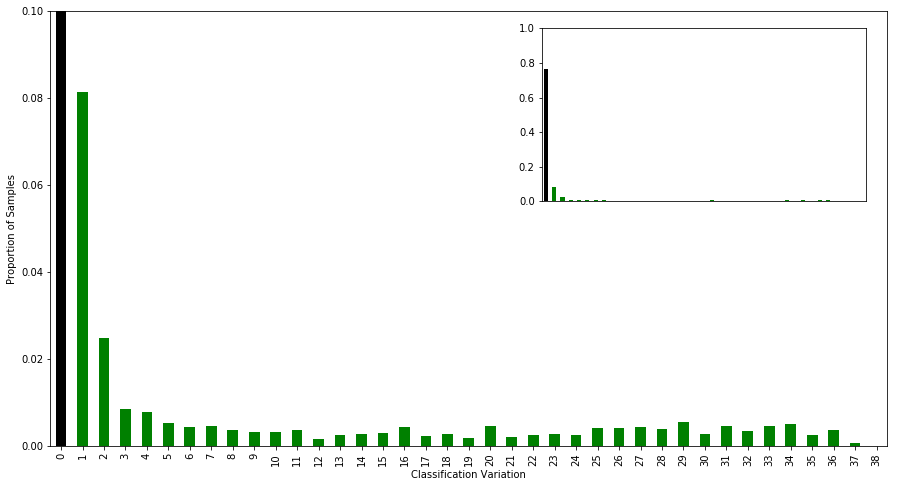
\includegraphics[width=0.95\textwidth]{Figures/distribution_clean.png}
	\caption[Distribution of duplicated samples with $\Pf=0$.]{Distribution of samples that started as goodware and changed in the number of positive classifications between the last and first submission, \ie $\Pl-\Pf$ for samples with $\Pf=0$}
	\label{fig:distribution_clean}
\end{figure}

With these minimum/maximum thresholds for malware/goodware we can now define our new metric $\Mac$ as:

\begin{itemize}
	\item $\tp_v$, \emph{true positive for $v$}, if $v$ and at least 5 other vendors in $\mathcal{V}$ classify it positively;
	\item $\tn_v$, \emph{true negative for $v$}, if $v$ and all other vendors in $\mathcal{V}$ classify it negatively;
	\item $\fp_v$, \emph{false positive for $v$}, if $v$ is the only vendor in $\mathcal{V}$ classifying it positively;
	\item $\fn_v$, \emph{false negative for $v$}, if $v$ classifies it negatively and at least 5 other vendors in $\mathcal{V}$ classify it positively.
\end{itemize}

Having the new metric defined, we again plot each vendors' $\dr_v$ vs.\ $\fpr_v$ according to~$\Mac$, presented in Figure \ref{fig:dr_fpr_d}.
Using this metric we note that vendors' detection rate is more scattered than under $\Madups$, ranging from 20.17\% to 83.50\%, whereas false positive rate is similar, ranging from 0.01\% to 5.77\%.
The scattering along the \tpr\ axis is not surprising, as now we are measuring each vendor $v$ against all others.
What is surprising is the amount of vendors below 50\% detection rate under this metric.
Possible reasoning behind this is either vendors disagree on what is malware (\ie\ \textit{ground truth} problem), or some vendors simply are not good at detecting malware.
As for the \fpr\ axis, it is still interesting to note how the scale remains relatively small, again reflecting the false negative over false positive preference.

\begin{figure}[!htb]
	\centering
	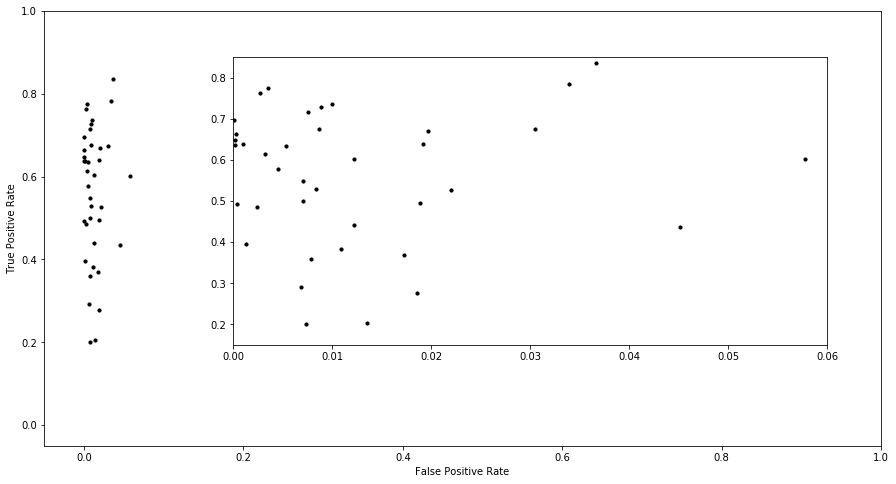
\includegraphics[width=0.95\textwidth]{Figures/dr_fpr_d.png}
	\caption{$\tpr_v$ vs. $\fpr_v$ according to $\Mac$.}
	\label{fig:dr_fpr_d}
\end{figure}

After studying vendors' accuracy under our defined metrics, and given the impossibility of finding a source that is able to unanimously label each sample in our dataset, we want to find the vendors that perform the best under both metrics $\Madups$ and $\Mac$.

Our approach to this problem is to filter the top 20 vendors $\VVdups$ and $\VVc$, according to each metric and define $\VVstar=\VVdups\cap\VVc$.
Given we have to maximize two variables, \tpr\ and \fpr, we decided to take advantage of the linear equation in the form $mx+b=y$ to choose the top vendors.
This form allows us to choose an $m$ and $b$ such that there are 20 vendors above the line, the top vendors $\VVstar$.
By tweaking the variable $m$ one can change the line's steepness, reflecting in a preference between \tpr\ and \fpr\:

\begin{itemize}
	\item \tpr\ preference: $m < 1$, less steepness therefore higher \fpr\ and \tpr\ values;
	\item \fpr\ preference: $m > 1$, more steepness, lower \fpr\ and \tpr\ values.
\end{itemize}

Since we have no \emph{a priori} preference between $\tpr$ nor $\fpr$, we search for the maximum $b$ with $m=1$ such that there are exactly 20 vendors above $x+b=y$ in each graphic (Figures~\ref{fig:dr_fpr_own} and~\ref{fig:dr_fpr_d}).

Figure \ref{fig:dr_fpr_top} shows the $\dr_v$ vs. $\fpr_v$ for the resulting 11 vendors under each metric, $\Madups$ in green and $\Mac$ in red, with $\dr_v$ varying from 63.49\% to 83.50\% and $\fpr_v$ from 0.01\% to 3.67\%.

\begin{figure}[!h]
	\centering
	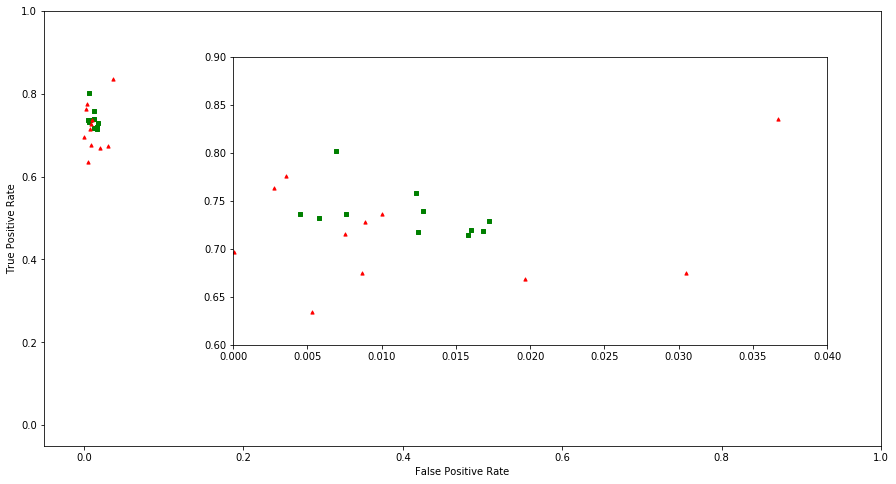
\includegraphics[width=\columnwidth]{Figures/dr_fpr_top.png}
	\caption{$\tpr_v$ vs. $\fpr_v$ according to $\Madups$ (green) and $\Mac$ (red).}
	\label{fig:dr_fpr_top}
\end{figure}

With a better understanding on the vendors' accuracy, followed by metrics that allowed us to narrow down the amount of vendors to those that perform best under our metrics, we can now proceed to label our samples as either goodware or malware.

%%%%%%%%%%%%%%%%%%%%%%%%%%%%%%%%%%%%%%%%%%%%%%%%%%%%%%%%%%%%%%%%%%%%%%%%
\section{Data labeling}
\label{section:data_labeling}

Given we are interested not only in providing a model to detect malware, but also in understanding the impacts of \textit{ground truth} in a detection model, we now go into detail on how we made use of the previously defined top vendors $\VVstar$ in conjunction with the information provided by \gls{nsrl} and VirusShare.com to label the available samples.
To do so, we take the previously defined scenarios in Figure \ref{fig:dataset_sizes} to define three labeling metrics.

The first and most real metric we define is $\Mrealv$ that labels a sample $s\in\CC$ as:

\begin{itemize}
	\item $s\in\mal_\real$ if at least 5 vendors in $\VVstar$ classify $s$ positively;
	\item $s\in\good_\real$ if all vendors in $\VVstar$ classify $s$ negatively.
\end{itemize}

Since the labeling information is solely provided by $\VVstar$'s vendors, this metric's ground truth is highly dependent on their performance, which means labeling errors may be present (as we have discussed in \ref{subsection:virustotal_classifications}).
To minimize this dependency, samples between one and four positive classifications are discarded.

\medskip

Our second metric $\Mloosev$, restricts the previous metric $\Mrealv$ to achieve a better ground truth and takes into account the information from \gls{nsrl}, defined by the set $\CNSRL=\NSRL\ \cap\ \CC$, and VirusShare.com, defined by the set $\CVS=\VS\ \cap\ \CC$.

This metric labels a sample $s\in\mathcal{C}$ as:
\begin{itemize}
	\item $s\in\mal_\loose$ if $s\in\mal_\real$ \textbf{and} it belongs to $\CVS$ and does not belong to $\CNSRL$;
	\item $s\in\good_\loose$ if $s\in\good_\real$ \textbf{and} it belongs to $\CNSRL$ and does not belong to $\CVS$.
\end{itemize}
that is
\begin{eqnarray*}
	\mal_\loose&=&\left(\mal_\real\cap\CVS\right)\setminus\CNSRL\\
	\good_\loose&=&\left(\good_\real\cap\CNSRL\right)\setminus\CVS
\end{eqnarray*}

By taking into account the presence in $\NSRL$, that reinforces cleanliness, and VirusShare.com, that reinforces maliciousness, this metric is more reliable, ground truth wise, at the expense of a smaller number of samples.
% (since $\DNSRL \subset\DD$ and $\DVS \subset \DD$).

\medskip

Our third and final metric $\Mstrictv$, is the strictest one, labeling a sample $s\in\CC$ as:
\begin{itemize}
	\item $s\in\mal_\strict$ if all $v\in\VVstar$ classify it positively \textbf{and} $s\in\CVS\setminus\CNSRL$;
	\item $s\in\good_\strict$ if $s\in\good_\loose$.
\end{itemize}

Obviously this is the most reliable metric, in the sense that it is closely related to the samples' ground truth, leaving little room for disagreement. However, this is achieved again at the cost of a smaller number of samples.

Having these three metrics for labeling, we can now proceed to create the datasets for each of these metrics.

%%%%%%%%%%%%%%%%%%%%%%%%%%%%%%%%%%%%%%%%%%%%%%%%%%%%%%%%%%%%%%%%%%%%%%%%
\section{Dataset creation}
\label{section:dataset_creation}

Taking the previously defined metrics, the task of creating labeled datasets based on them is trivial.
We apply each of the previously defined metrics, $\Mstrictv$, $\Mloosev$ and $\Mrealv$ to our classified dataset $\CC$ to obtained three new datasets, $\CC_{strict}\subseteq\CC_{loose}\subseteq\CC_{real}\subseteq\CC$.
Table \ref{tab:dataset_sizes} provides information regarding the size and number of malware and goodware in each of our datasets.

\begin{table}[!htb]
	\renewcommand{\arraystretch}{1.2} % more space between rows
	\centering
	\begin{tabular}{lccc}
		\toprule
		Dataset			& $\CC_{real}$ & $\CC_{loose}$ & $\CC_{strict}$	\\
		\midrule
		Malware			& 0 & 0 & 0\\
		Goodware		& 0 & 0 & 0\\
		\midrule
		Total			& 0 & 0 & 0\\
		\bottomrule
	\end{tabular}
	\caption{Sizes for datasets $\CC_{real}$, $\CC_{loose}$ and $\CC_{strict}$.}
	\label{tab:dataset_sizes}
\end{table}

\medskip

In this chapter we analyzed our available data in order to better understand its advantages and disadvantages.
We provided information regarding our data sources and how the extraction process was made, followed how a simple high level analysis provided interesting insights on the available data.

We took some time understanding how vendors classified reports, how they changed their classifications and how it could impact the reliability of our labels - so much so we defined different metrics that provide different levels of \textit{ground truth} reliability.

Out of these metrics we created three datasets, all subsets of $\CC$, in hopes of enlightening the impacts of \textit{ground truth} when it comes to the task of detecting malware. We are now ready to make use of the datasets to build a malware detection model, which will take place in the following chapters.
